%{{{ prelude
\documentclass{beamer}
\usepackage[T1]{fontenc}
\usepackage[math]{iwona}
\usepackage{hyperref}
\usepackage{pgfpages}
\usepackage{tikz}
\usepackage{graphicx}
\usepackage{xspace}

\setbeamertemplate{navigation symbols}{}
\setbeamercolor{normal text}{bg=black,fg=white}
\setbeamercolor{alerted text}{fg=yellow}
\setbeamercolor{structure}{fg=green}

\newcommand{\titletext}{The Design and Algorithms of a Verification Condition
  Generator}
\definecolor{lightblue}{rgb}{0.5,0.5,1}
\hypersetup{colorlinks,linkcolor=lightblue,citecolor=lightblue,urlcolor=lightblue}
\hypersetup{
  pdfauthor={Radu Grigore},
  pdftitle={\titletext}}

\tikzset{statement/.style={
  rectangle,
  draw,thick,
  inner sep=2pt,minimum height=3ex}}
\tikzset{>=latex}
\tikzset{shorten >=1pt}

\title{\titletext}
\author{Radu Grigore}
\date{23 August 2010}

\newcommand{\specsharp}{Spec$^\sharp$\xspace}
\newcommand{\limp}{\Rightarrow}
\newcommand{\tru}{\top}
%}}} prelude

\begin{document}
\maketitle
%{{{ plan
% Audience: Rustan and Henry.
% Principles:
%   - give a good overview
%     - spend plenty of time explaining how pieces fit together
%     - mention all the contributions explicitly
%   - go in depth into one subject (say, reachability)
% Plan
%   - here's the field and why it's interesting
%   - here's what I did and why it's important
%   - here's some clever details
%   - 
% Extra slides (for answering questions):
%   - TODO 
%}}}
%{{{ motivation
\begin{frame}
  \begin{block}{formal methods}
  \begin{itemize}
  \item use mathematics to improve the quality of software
  \item directions
    \begin{itemize}
    \item how should humans think about programs
    \item how should machines think about programs
    \end{itemize}
  \item appealing because
    \begin{itemize}
    \item potentially very useful
    \item many small beautiful problems
    \end{itemize}
  \end{itemize}
  \end{block}

  \begin{block}{program verifiers}
  \begin{itemize}
  \item high quality new code
  \item fix problems in old code
  \end{itemize}
  \end{block}
\end{frame}
%}}}
%{{{ contributions
\begin{frame}
  \begin{block}{\specsharp architecture}
  \begin{itemize}
  \item \specsharp compiler (frontend)
  \item Boogie tool (backend)
    \begin{itemize}
    \item \emph{verification condition generator}
    \item SMT solver
    \end{itemize}
  \end{itemize}
  \end{block}
  \begin{block}{improvements}
  \begin{itemize}
  \item \alert{incremental}
  \item \alert{analysis} of finding a passive form
  \item \alert{configurable method}
    \begin{itemize}
    \item weakest precondition
    \item strongest postcondition
    \end{itemize}
  \item analyzes
    \begin{itemize}
    \item partial correctness
    \item \alert{reachability}
    \end{itemize}
  \end{itemize}
  \end{block}
\end{frame}
%}}}
%{{{ Boogie example
\newcommand{\sequentialsearch}[1]{
  \begin{tikzpicture}[x={(2.25cm,0cm)},y={(0cm,-1cm)}]
    \def\prop##1{\ifnum#1=##1yellow\fi}
    \foreach \n/\p/\l in {
        0/{(0,0)}/{$i:=0$},
        1/{(-1,1)}/{\textbf{assume} $i<n\land v[i]\ne u$},
        2/{(-1,2)}/{$i:=i+1$},
        3/{(1,1)}/{\textbf{assume} $i\ge n\lor v[i]=u)$},
        4/{(1,2)}/{\textbf{assert} $v[i]=u$},
        5/{(1,3)}/{\textbf{return}} }
      \node[statement,\prop\n] (\n) at \p {\l};
    \draw[->] (2) .. controls (-2.3,4.5) and (-2.3,-1.5) ..  (1);
    \foreach \m/\n in {0/1,0/3,1/2,2/3,3/4,4/5}
      \draw[->] (\m)--(\n);
  \end{tikzpicture}}

\begin{frame}
\begin{align*}
\\
\end{align*}
\begin{center}
  \sequentialsearch9
\end{center}
\end{frame}

\begin{frame}
\begin{align*}
\\
  \alert{\sigma_0=[i\mapsto7,v\mapsto[9,8,6],n\mapsto3,u\mapsto8]}
\end{align*}
\begin{center}
  \sequentialsearch0
\end{center}
\end{frame}

\begin{frame}
\begin{align*}
  \sigma_0=[i\mapsto7,v\mapsto[9,8,6],n\mapsto3,u\mapsto8]
\\
  \alert{\sigma_1=[i\mapsto0,v\mapsto[9,8,6],n\mapsto3,u\mapsto8]}
\end{align*}
\begin{center}
  \sequentialsearch1
\end{center}
\end{frame}

\begin{frame}
\begin{align*}
  \sigma_0=[i\mapsto7,v\mapsto[9,8,6],n\mapsto3,u\mapsto8]
\\
  \alert{\sigma_1=[i\mapsto0,v\mapsto[9,8,6],n\mapsto3,u\mapsto8]}
\end{align*}
\begin{center}
  \sequentialsearch2
\end{center}
\end{frame}

\begin{frame}
\begin{align*}
  \sigma_1=[i\mapsto0,v\mapsto[9,8,6],n\mapsto3,u\mapsto8]
\\
  \alert{\sigma_2=[i\mapsto1,v\mapsto[9,8,6],n\mapsto3,u\mapsto8]}
\end{align*}
\begin{center}
  \sequentialsearch3
\end{center}
\end{frame}

\begin{frame}
\begin{align*}
  \sigma_1=[i\mapsto0,v\mapsto[9,8,6],n\mapsto3,u\mapsto8]
\\
  \alert{\sigma_2=[i\mapsto1,v\mapsto[9,8,6],n\mapsto3,u\mapsto8]}
\end{align*}
\begin{center}
  \sequentialsearch4
\end{center}
\end{frame}

\begin{frame}
\begin{align*}
  \sigma_1=[i\mapsto0,v\mapsto[9,8,6],n\mapsto3,u\mapsto8]
\\
  \alert{\sigma_2=[i\mapsto1,v\mapsto[9,8,6],n\mapsto3,u\mapsto8]}
\end{align*}
\begin{center}
  \sequentialsearch5
\end{center}
\end{frame}

\begin{frame}
\begin{align*}
\\
  \alert{\sigma_0=[i\mapsto7,v\mapsto[9,8,6],n\mapsto3,u\mapsto8]}
\end{align*}
\begin{center}
  \sequentialsearch0
\end{center}
\end{frame}

\begin{frame}
\begin{align*}
  \sigma_0=[i\mapsto7,v\mapsto[9,8,6],n\mapsto3,u\mapsto8]
\\
  \alert{\sigma_1=[i\mapsto0,v\mapsto[9,8,6],n\mapsto3,u\mapsto8]}
\end{align*}
\begin{center}
  \sequentialsearch3
\end{center}
\end{frame}

\begin{frame}
\begin{align*}
\\
  \alert{\sigma_0=[i\mapsto7,v\mapsto[9,8,6],n\mapsto0,u\mapsto8]}
\end{align*}
\begin{center}
  \sequentialsearch0
\end{center}
\end{frame}

\begin{frame}
\begin{align*}
  \sigma_0=[i\mapsto7,v\mapsto[9,8,6],n\mapsto0,u\mapsto8]
\\
  \alert{\sigma_1=[i\mapsto0,v\mapsto[9,8,6],n\mapsto0,u\mapsto8]}
\end{align*}
\begin{center}
  \sequentialsearch3
\end{center}
\end{frame}

\begin{frame}
\begin{align*}
  &\sigma_0=[i\mapsto7,v\mapsto[9,8,6],n\mapsto0,u\mapsto8]
\\
  &\alert{\sigma_1=[i\mapsto0,v\mapsto[9,8,6],n\mapsto0,u\mapsto8]}
\end{align*}
\begin{center}
  \sequentialsearch4
\end{center}
\end{frame}

\begin{frame}
\begin{align*}
  &\sigma_1=[i\mapsto0,v\mapsto[9,8,6],n\mapsto0,u\mapsto8]
\\
  &\alert{\textit{error}}
\end{align*}
\begin{center}
  \sequentialsearch9
\end{center}
\end{frame}
%}}} Boogie example
% {{{ Boogie semantics
\begin{frame}
\begin{align*}
  &\langle\sigma_0,x_0\rangle\leadsto
  \langle\sigma_1,x_1\rangle\leadsto
  \langle\sigma_2,x_2\rangle\leadsto
  \cdots\leadsto
  \langle\sigma_n,x_n\rangle
\\
  &\langle\sigma_0,x_0\rangle\leadsto
  \langle\sigma_1,x_1\rangle\leadsto
  \langle\sigma_2,x_2\rangle\leadsto
  \cdots\leadsto
  \langle\sigma_n,x_n\rangle\leadsto
  \mathit{error}
\end{align*}

\pause
$$\frac
  {\text{$x$ is $v:=e$}\quad x\to x'\quad \sigma'=(v\gets e)\;\sigma}
  {\langle\sigma,x\rangle\leadsto\langle\sigma',x'\rangle}$$
$$\frac
  {\text{$x$ is \textbf{assert}~$q$}\quad x\to x'\quad q(\sigma)}
  {\langle\sigma,x\rangle\leadsto\langle\sigma,x'\rangle}$$
\end{frame}

\begin{frame}
a Boogie program is \alert{partially correct}
$$\iff$$
it has no execution that \alert{goes wrong}
$$\iff$$
it is possible to attach a precondition~$a_x$ and a postcondition~$b_x$
to each statement~$x$ such that
\begin{itemize}
\item $|a_0|$,
\item $\{a_x\}\;x\;\{b_x\}$ for all statements~$x$, and
\item $|b_x\limp a_y|$ if $x\to y$.
\end{itemize}

where
\begin{align*}
\{p\}\;\textbf{assert~$q$}\;\{r\} &= \bigl|p\limp(q\land r)\bigr| \\
\{p\}\;\textbf{assume~$q$}\;\{r\} &= \bigl|(p\land q)\limp r\bigr| \\
\end{align*}
\end{frame}


\begin{frame}
  \frametitle{\textbf{return} $x|1$}
\begin{center}
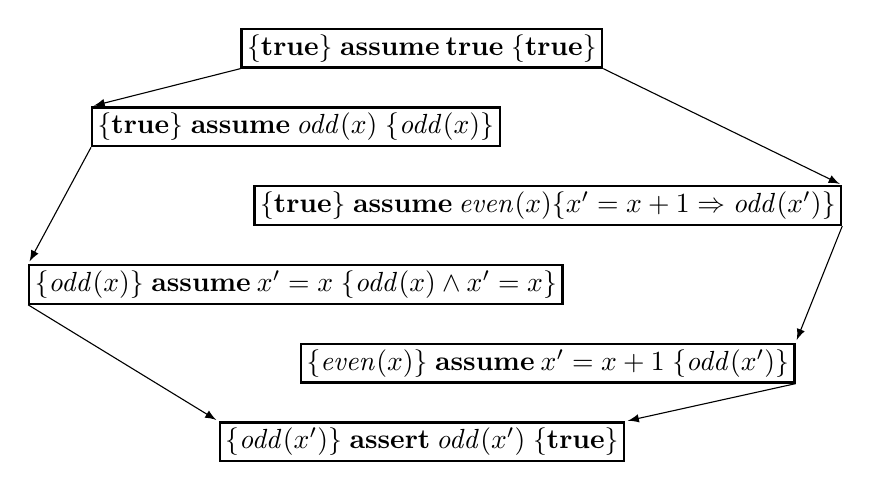
\begin{tikzpicture}[x={(1.6cm,0cm)},y={(0cm,-1cm)}]
  \foreach \n/\p/\l in {
      0/{(0,0)}/{\{\mathbf{true}\}\;\textbf{assume}\>\mathbf{true}\;\{\mathbf{true}\}},
      1/{(-1,1)}/{\{\mathbf{true}\}\;\textbf{assume}\>\mathit{odd}(x)\;\{\mathit{odd}(x)\}},
      2/{(-1,3)}/{\{\mathit{odd}(x)\}\;\textbf{assume}\>x'=x\;\{\mathit{odd}(x)\land x'=x\}},
      3/{(1,2)}/{\{\mathbf{true}\}\;\textbf{assume}\>\mathit{even}(x)\{x'=x+1\limp\mathit{odd}(x')\}},
      4/{(1,4)}/{\{\mathit{even}(x)\}\;\textbf{assume}\>x'=x+1\;\{\mathit{odd}(x')\}},
      5/{(0,5)}/{\{\mathit{odd}(x')\}\;\textbf{assert}\>\mathit{odd}(x')\;\{\mathbf{true}\}} }
    \node[statement] (\n) at \p {$\l$};
  \foreach \m/\n in {0/1,1/2,2/5}
    \draw[->] (\m.south west) -- (\n.north west);
  \foreach \m/\n in {0/3,3/4,4/5}
    \draw[->] (\m.south east) -- (\n.north east);
\end{tikzpicture}
\end{center}
\end{frame}

\begin{frame}
  \begin{block}{weakest precondition}
  \begin{align*}
  b_x &\equiv \textstyle\bigwedge_{x\to y} a_y \\
  a_x &\equiv 
    \begin{cases}
    q_x\limp b_x & \text{if $x$ is \textbf{assume} $q_x$} \\
    q_x\land b_x & \text{if $x$ is \textbf{assert} $q_x$}
    \end{cases}\\
  \mathit{vc} &\equiv a_0
  \end{align*}
  \end{block}
  \begin{block}{strongest postcondition}
  \begin{align*}
  a_y &\equiv
    \begin{cases}
    \tru & \text{if $y$ is the initial statement} \\
    \bigvee_{x\to y} b_x & \text{otherwise}
    \end{cases} \\
  b_y &\equiv a_y \land q_y \qquad\text{where $y$ is \textbf{assume/assert} $q_y$} \\
  \mathit{vc} &\equiv \textstyle\bigwedge_\text{$y$ is \textbf{assert} $q_y$} (a_y\limp q_y)
  \end{align*}
  \end{block}
\end{frame}

% {{{ wp example
\begin{frame}
  \frametitle{weakest precondition for $\mathbf{return}\>\mathit{abs}(x)$}
\begin{center}
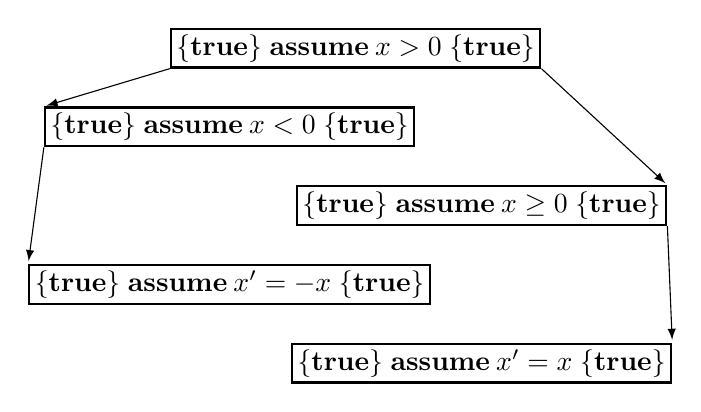
\begin{tikzpicture}[x={(1.6cm,0cm)},y={(0cm,-1cm)}]
  \foreach \n/\p/\l in {
      1/{(-1,1)}/{x<0},
      2/{(-1,3)}/{x'=-x},
      3/{(1,2)}/{x\ge 0},
      4/{(1,4)}/{x'=x}}
    \node[statement] (\n) at \p {$\{\mathbf{true}\}\;\mathbf{assume}\>\l\;\{\mathbf{true}\}$};
  \node [statement] (0) at (0,0) {$\{\alert{\mathbf{true}}\}\;\mathbf{assume}\>x>0\;\{\mathbf{true}\}$};
  \foreach \m/\n in {0/1,1/2}
    \draw[->] (\m.south west) -- (\n.north west);
  \foreach \m/\n in {0/3,3/4}
    \draw[->] (\m.south east) -- (\n.north east);
\end{tikzpicture}
\end{center}
\end{frame}

\begin{frame}
  \frametitle{weakest precondition for $\mathbf{return}\>\mathit{abs}(x)$}
\begin{center}
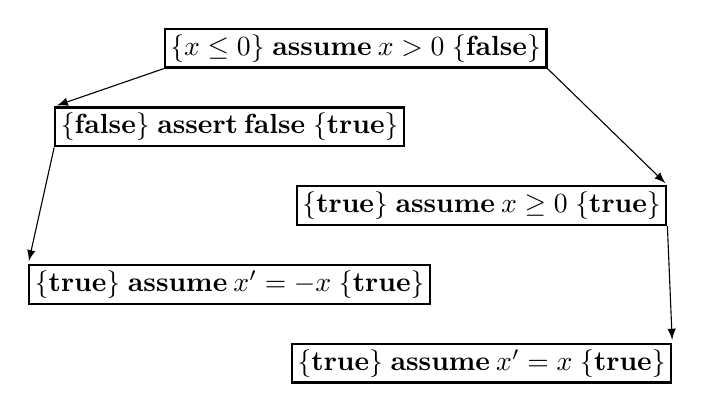
\begin{tikzpicture}[x={(1.6cm,0cm)},y={(0cm,-1cm)}]
  \foreach \n/\p/\l in {
      0/{(0,0)}/{\{\alert{x\le0}\}\;\mathbf{assume}\>x>0\;\{\mathbf{false}\}},
      1/{(-1,1)}/{\{\mathbf{false}\}\;\mathbf{assert}\>\mathbf{false}\;\{\mathbf{true}\}},
      2/{(-1,3)}/{\{\mathbf{true}\}\;\mathbf{assume}\>x'=-x\;\{\mathbf{true}\}},
      3/{(1,2)}/{\{\mathbf{true}\}\;\mathbf{assume}\>x\ge 0\;\{\mathbf{true}\}},
      4/{(1,4)}/{\{\mathbf{true}\}\;\mathbf{assume}\>x'=x\;\{\mathbf{true}\}} }
    \node[statement] (\n) at \p {$\l$};
  \foreach \m/\n in {0/1,1/2}
    \draw[->] (\m.south west) -- (\n.north west);
  \foreach \m/\n in {0/3,3/4}
    \draw[->] (\m.south east) -- (\n.north east);
\end{tikzpicture}
\end{center}
\end{frame}

\begin{frame}
  \frametitle{weakest precondition for $\mathbf{return}\>\mathit{abs}(x)$}
\begin{center}
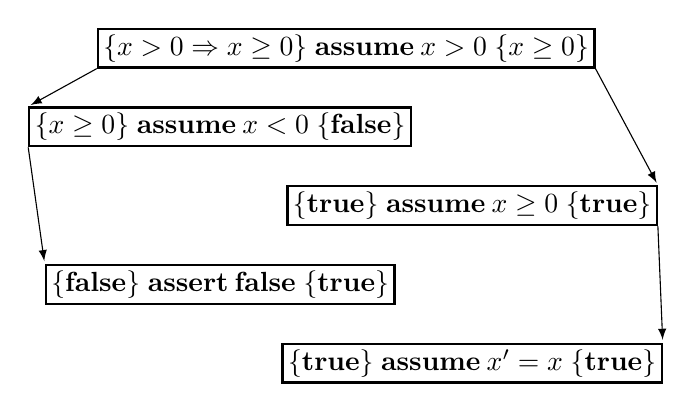
\begin{tikzpicture}[x={(1.6cm,0cm)},y={(0cm,-1cm)}]
  \foreach \n/\p/\l in {
      0/{(0,0)}/{\{\alert{x>0\limp x\ge0}\}\;\mathbf{assume}\>x>0\;\{x\ge0\}},
      1/{(-1,1)}/{\{x\ge0\}\;\mathbf{assume}\>x<0\;\{\mathbf{false}\}},
      2/{(-1,3)}/{\{\mathbf{false}\}\;\mathbf{assert}\>\mathbf{false}\;\{\mathbf{true}\}},
      3/{(1,2)}/{\{\mathbf{true}\}\;\mathbf{assume}\>x\ge 0\;\{\mathbf{true}\}},
      4/{(1,4)}/{\{\mathbf{true}\}\;\mathbf{assume}\>x'=x\;\{\mathbf{true}\}} }
    \node[statement] (\n) at \p {$\l$};
  \foreach \m/\n in {0/1,1/2}
    \draw[->] (\m.south west) -- (\n.north west);
  \foreach \m/\n in {0/3,3/4}
    \draw[->] (\m.south east) -- (\n.north east);
\end{tikzpicture}
\end{center}
\end{frame}
% }}} wp example
% {{{ sp example
\begin{frame}
  \frametitle{strongest postcondition for $\mathbf{return}\>\mathit{abs}(x)$}
\begin{center}
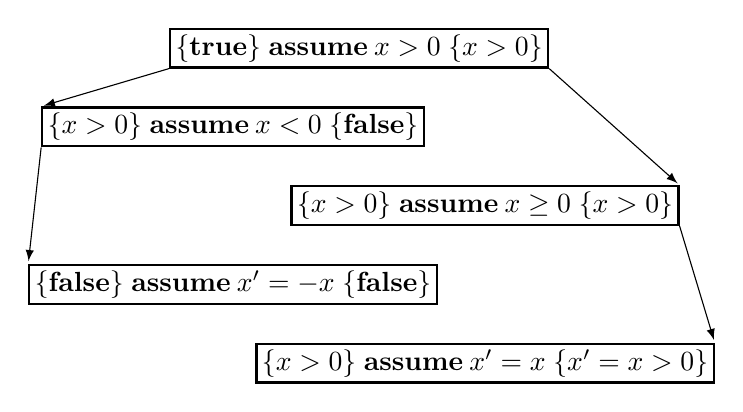
\begin{tikzpicture}[x={(1.6cm,0cm)},y={(0cm,-1cm)}]
  \foreach \n/\p/\l in {
      0/{(0,0)}/{\{\mathbf{true}\}\;\mathbf{assume}\>x>0\;\{x>0\}},
      1/{(-1,1)}/{\{x>0\}\;\mathbf{assume}\>x<0\;\{\mathbf{false}\}},
      2/{(-1,3)}/{\{\mathbf{false}\}\;\mathbf{assume}\>x'=-x\;\{\mathbf{false}\}},
      3/{(1,2)}/{\{x>0\}\;\mathbf{assume}\>x\ge 0\;\{x>0\}},
      4/{(1,4)}/{\{x>0\}\;\mathbf{assume}\>x'=x\;\{x'=x>0\}} }
    \node[statement] (\n) at \p {$\l$};
  \foreach \m/\n in {0/1,1/2}
    \draw[->] (\m.south west) -- (\n.north west);
  \foreach \m/\n in {0/3,3/4}
    \draw[->] (\m.south east) -- (\n.north east);
\end{tikzpicture}

$$\alert{\mathit{vc}\equiv\tru}$$
\end{center}
\end{frame}

\begin{frame}
  \frametitle{strongest postcondition for $\mathbf{return}\>\mathit{abs}(x)$}
\begin{center}
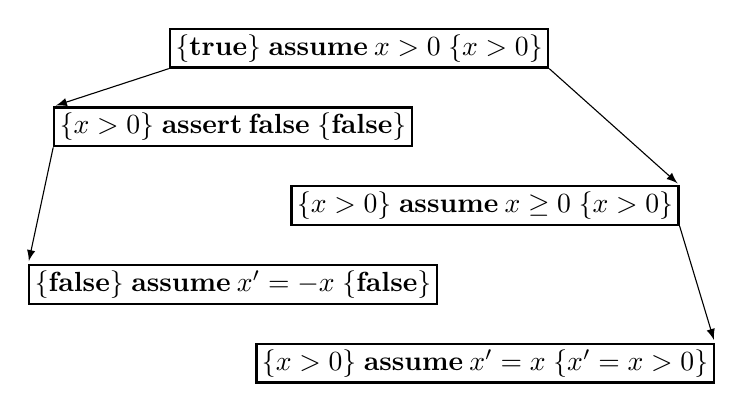
\begin{tikzpicture}[x={(1.6cm,0cm)},y={(0cm,-1cm)}]
  \foreach \n/\p/\l in {
      0/{(0,0)}/{\{\mathbf{true}\}\;\mathbf{assume}\>x>0\;\{x>0\}},
      1/{(-1,1)}/{\{\alert{x>0}\}\;\mathbf{assert}\>\alert{\mathbf{false}}\;\{\mathbf{false}\}},
      2/{(-1,3)}/{\{\mathbf{false}\}\;\mathbf{assume}\>x'=-x\;\{\mathbf{false}\}},
      3/{(1,2)}/{\{x>0\}\;\mathbf{assume}\>x\ge 0\;\{x>0\}},
      4/{(1,4)}/{\{x>0\}\;\mathbf{assume}\>x'=x\;\{x'=x>0\}} }
    \node[statement] (\n) at \p {$\l$};
  \foreach \m/\n in {0/1,1/2}
    \draw[->] (\m.south west) -- (\n.north west);
  \foreach \m/\n in {0/3,3/4}
    \draw[->] (\m.south east) -- (\n.north east);
\end{tikzpicture}

$$\alert{\mathit{vc}\equiv x\le0}$$
\end{center}
\end{frame}

\begin{frame}
  \frametitle{strongest postcondition for $\mathbf{return}\>\mathit{abs}(x)$}
\begin{center}
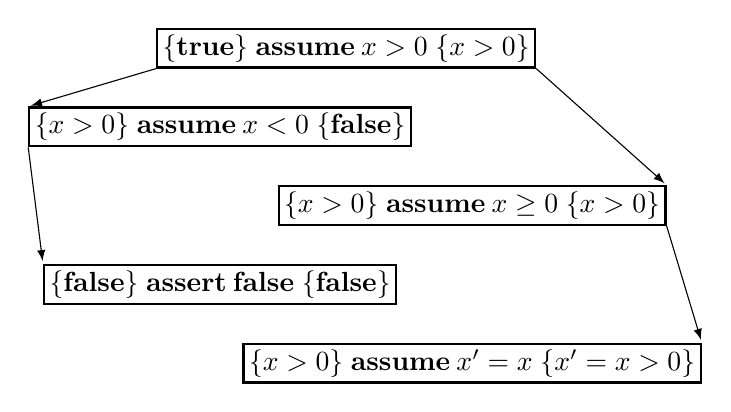
\begin{tikzpicture}[x={(1.6cm,0cm)},y={(0cm,-1cm)}]
  \foreach \n/\p/\l in {
      0/{(0,0)}/{\{\mathbf{true}\}\;\mathbf{assume}\>x>0\;\{x>0\}},
      1/{(-1,1)}/{\{x>0\}\;\mathbf{assume}\>x<0\;\{\mathbf{false}\}},
      2/{(-1,3)}/{\{\alert{\mathbf{false}}\}\;\mathbf{assert}\>\alert{\mathbf{false}}\;\{\mathbf{false}\}},
      3/{(1,2)}/{\{x>0\}\;\mathbf{assume}\>x\ge 0\;\{x>0\}},
      4/{(1,4)}/{\{x>0\}\;\mathbf{assume}\>x'=x\;\{x'=x>0\}} }
    \node[statement] (\n) at \p {$\l$};
  \foreach \m/\n in {0/1,1/2}
    \draw[->] (\m.south west) -- (\n.north west);
  \foreach \m/\n in {0/3,3/4}
    \draw[->] (\m.south east) -- (\n.north east);
\end{tikzpicture}

$$\alert{\mathit{vc}\equiv\tru}$$
\end{center}
\end{frame}
% }}} sp example
\begin{frame}
  \frametitle{reachability queries}
\begin{center}
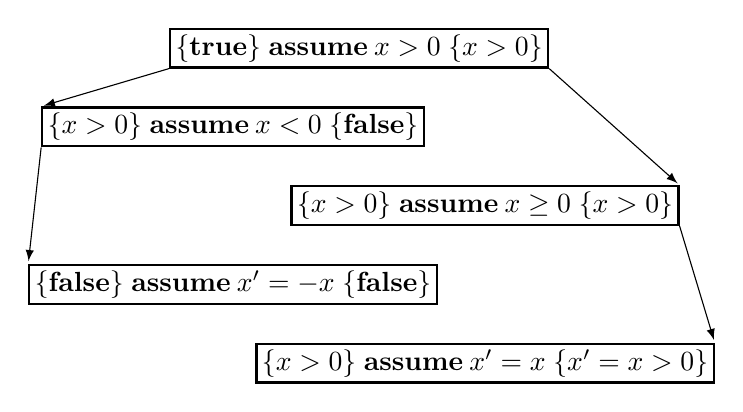
\begin{tikzpicture}[x={(1.6cm,0cm)},y={(0cm,-1cm)}]
  \foreach \n/\p/\l in {
      0/{(0,0)}/{\{\alert{\mathbf{true}}\}\;\mathbf{assume}\>x>0\;\{x>0\}},
      1/{(-1,1)}/{\{\alert{x>0}\}\;\mathbf{assume}\>x<0\;\{\mathbf{false}\}},
      2/{(-1,3)}/{\{\alert{\mathbf{false}}\}\;\mathbf{assume}\>x'=-x\;\{\mathbf{false}\}},
      3/{(1,2)}/{\{\alert{x>0}\}\;\mathbf{assume}\>x\ge 0\;\{x>0\}},
      4/{(1,4)}/{\{\alert{x>0}\}\;\mathbf{assume}\>x'=x\;\{x'=x>0\}} }
    \node[statement] (\n) at \p {$\l$};
  \foreach \m/\n in {0/1,1/2}
    \draw[->] (\m.south west) -- (\n.north west);
  \foreach \m/\n in {0/3,3/4}
    \draw[->] (\m.south east) -- (\n.north east);
\end{tikzpicture}
\end{center}
\end{frame}


% }}} Boogie semantics
%{{{ Q&A
\begin{frame}
\centerline{\Huge Q\&A}
\end{frame}
%}}}
%{{{ extra
\begin{frame}
  \frametitle{Contributions}
  \begin{itemize}
  \item semantics for core Boogie: operational, Hoare, wp, sp, relation
  \item novel use of Visitors, and the supporting tool AstGen; there's
    also a discussion of the overall design
  \item precise definition of passivation 
  \item study of the complexity of the passivation problem
  \item experimental comparison of wp vs sp
  \item algorithm for unsharing expression dags
  \item proof technique for algorithms that simplify verification conditions
  \item heuristic for detecting common parts of expression trees
  \item why is reachability analysis useful (in addition to correctness
    and termination)
  \item heuristics that make reachability analysis practical 
  \item FreeBoogie
  \end{itemize}
\end{frame}
%}}}
\end{document}

